\section{Introduction} \label{introduction}

Introduction to your report. Maybe you want to reference some publication~\cite{croft:2009}, just give the authors of some publication: \citeauthor{croft:2009}, or give the authors and the reference \citet{croft:2009}. Including graphics also is usually dead simple, like with Figure~\ref{rubber-duck}.

\begin{figure}[b]
    \centering
    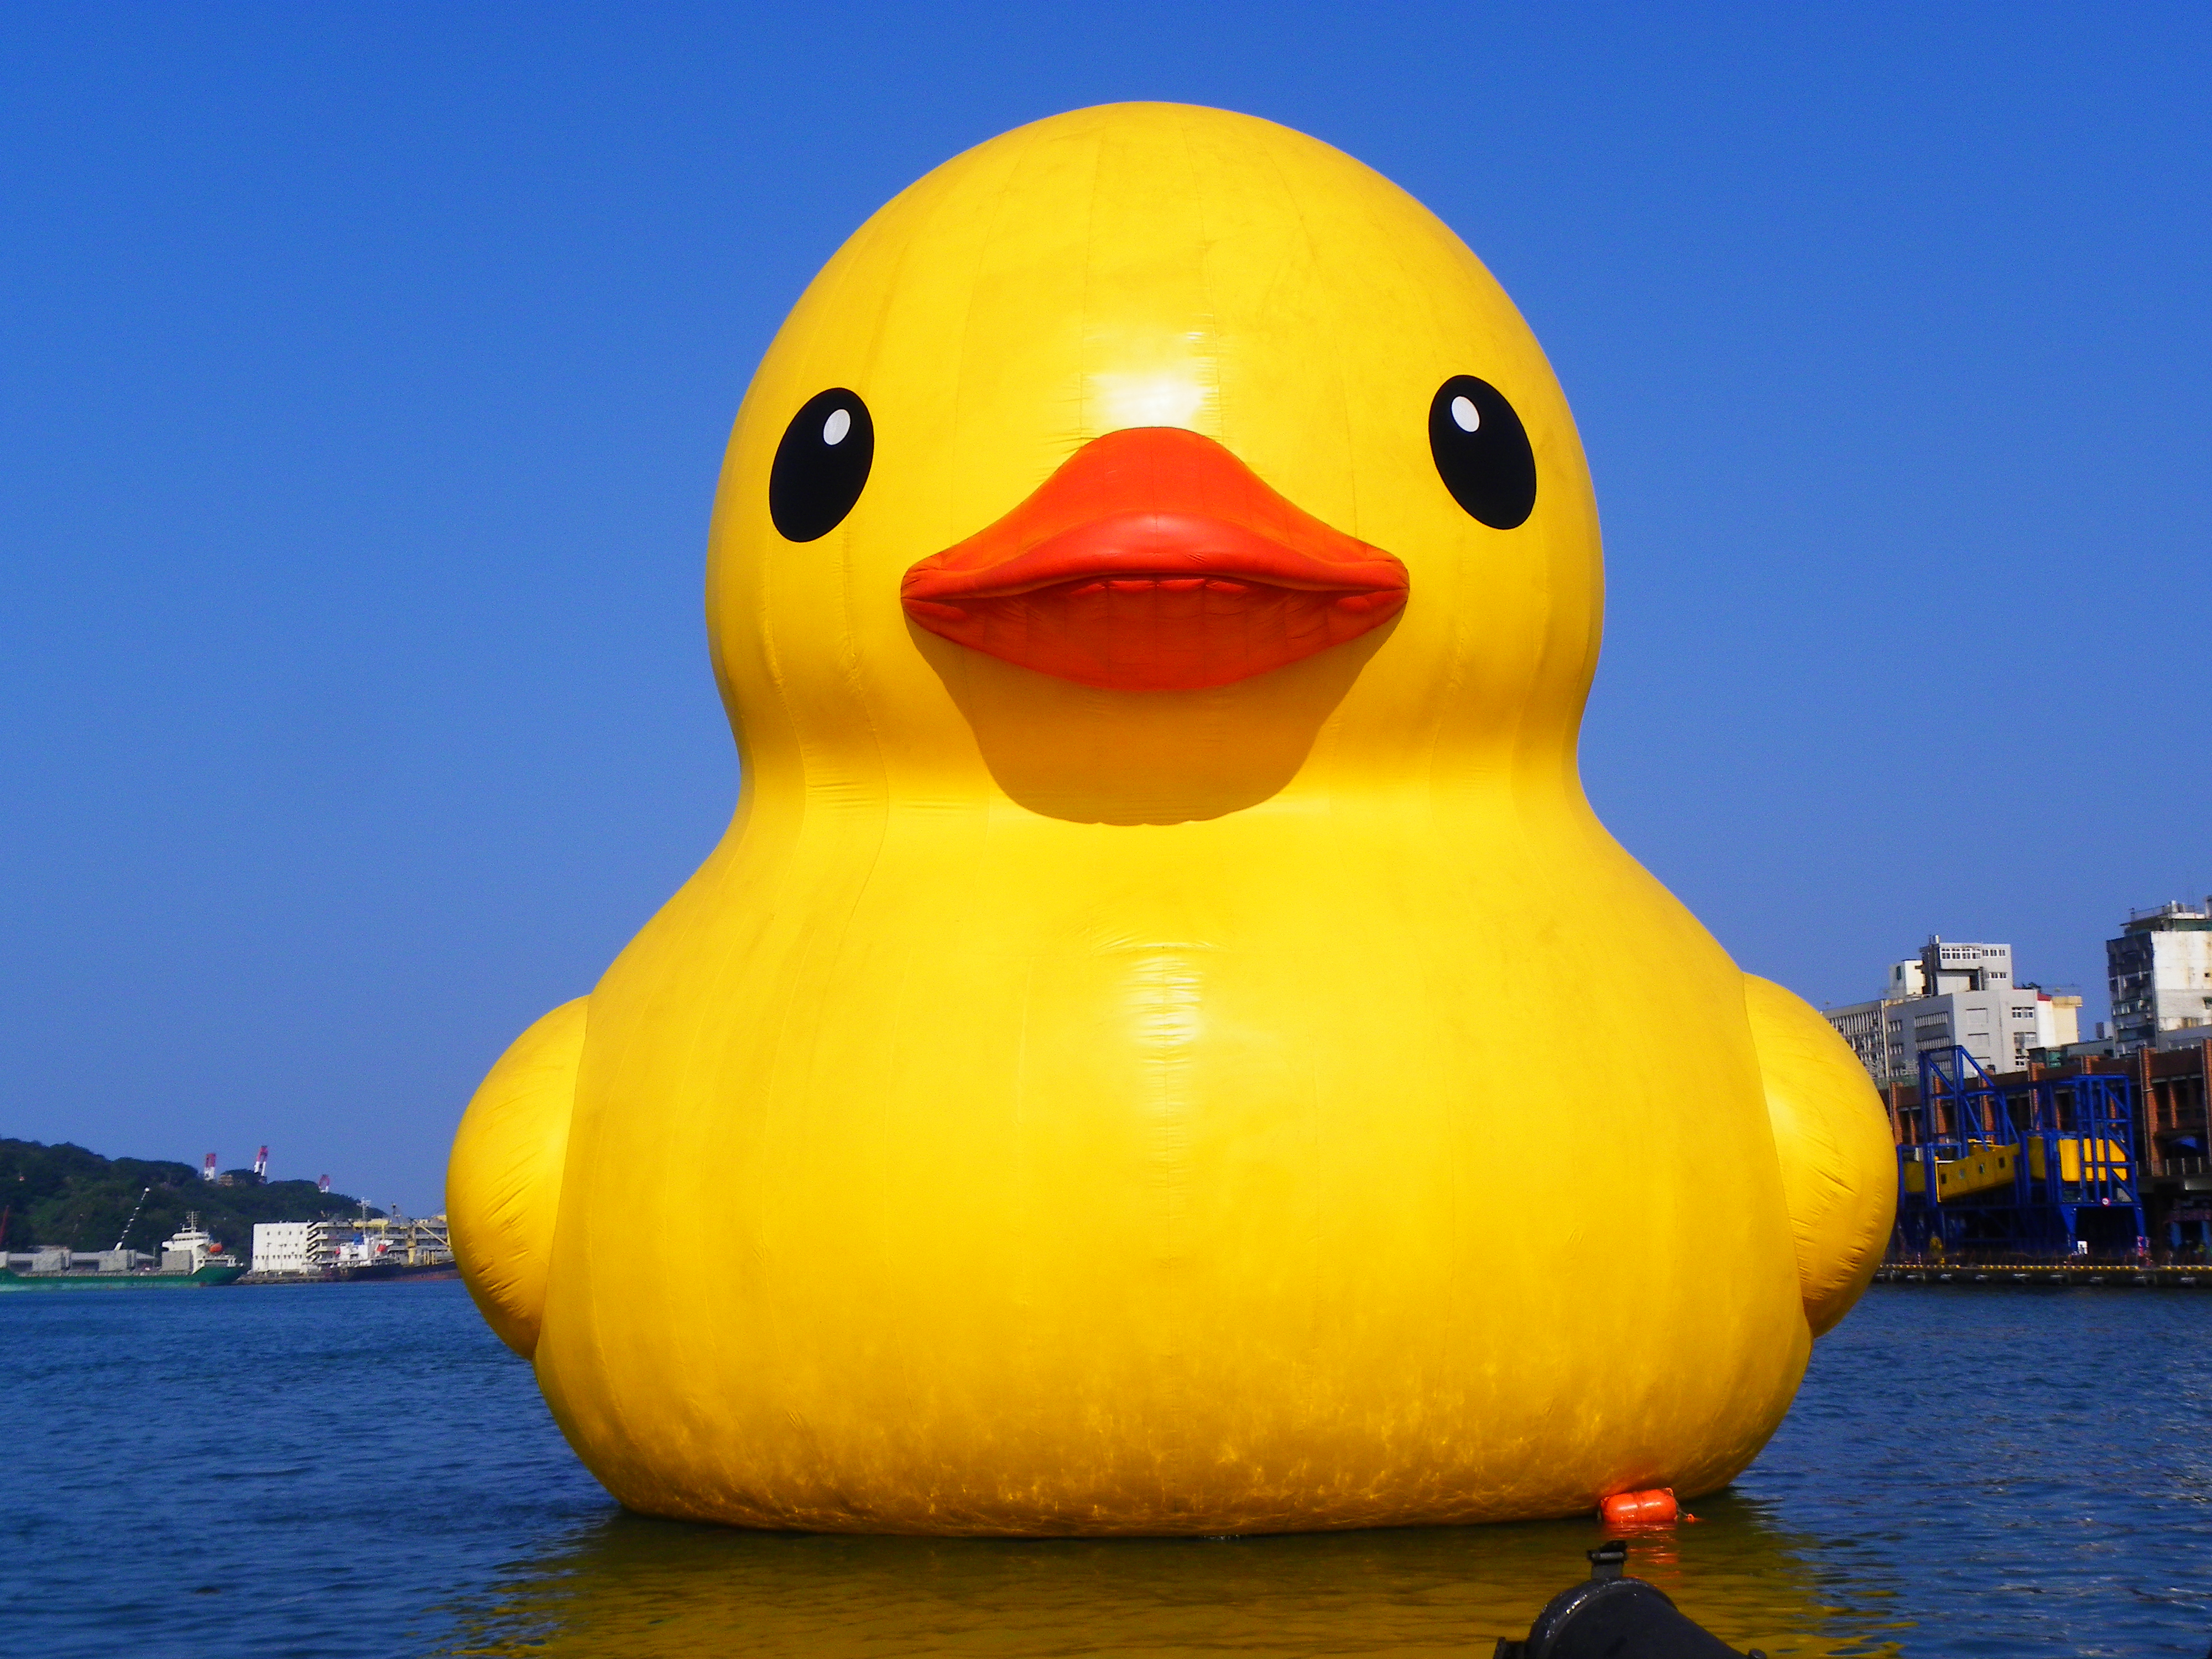
\includegraphics[width=\columnwidth]{rubber-duck}
    \caption{Some large rubber duck.}
    \Description{Floating large yellow rubber duck sculpture, designed by Dutch artist Florentijn Hofman. Image source: \url{https://commons.wikimedia.org/wiki/File:Rubber_Duck_Front_View_in_Fine_Day_20140107.jpg}.}
    \label{rubber-duck}
\end{figure}

